%%%%%%%%%%%%%%%%%%%%%%%%%%%%%%%%%%%%%%%%%
% Short Sectioned Assignment
% LaTeX Template
% Version 1.0 (5/5/12)
%
% This template has been downloaded from:
% http://www.LaTeXTemplates.com
%
% Original author:
% Frits Wenneker (http://www.howtotex.com)
%
% License:
% CC BY-NC-SA 3.0 (http://creativecommons.org/licenses/by-nc-sa/3.0/)
%
%%%%%%%%%%%%%%%%%%%%%%%%%%%%%%%%%%%%%%%%%

%----------------------------------------------------------------------------------------
%	PACKAGES AND OTHER DOCUMENT CONFIGURATIONS
%----------------------------------------------------------------------------------------

\documentclass[paper=a4, fontsize=11pt]{scrartcl} % A4 paper and 11pt font size 

\usepackage[T1]{fontenc} % Use 8-bit encoding that has 256 glyphs
\usepackage[english]{babel} % English language/hyphenation
\usepackage{amsmath,amsfonts,amsthm} % Math packages

\usepackage{sectsty} % Allows customizing section commands
%\allsectionsfont{\centering \normalfont\scshape} % Make all sections centered, the default font and small caps

\usepackage{fancyhdr} % Custom headers and footers
\pagestyle{fancyplain} % Makes all pages in the document conform to the custom headers and footers
\fancyhead{} % No page header - if you want one, create it in the same way as the footers below
\fancyfoot[L]{} % Empty left footer
\fancyfoot[C]{} % Empty center footer
\fancyfoot[R]{\thepage} % Page numbering for right footer
\renewcommand{\headrulewidth}{0pt} % Remove header underlines
\renewcommand{\footrulewidth}{0pt} % Remove footer underlines
\setlength{\headheight}{13.6pt} % Customize the height of the header

\numberwithin{equation}{section} % Number equations within sections (i.e. 1.1, 1.2, 2.1, 2.2 instead of 1, 2, 3, 4)
\numberwithin{figure}{section} % Number figures within sections (i.e. 1.1, 1.2, 2.1, 2.2 instead of 1, 2, 3, 4)
\numberwithin{table}{section} % Number tables within sections (i.e. 1.1, 1.2, 2.1, 2.2 instead of 1, 2, 3, 4)

\setlength\parindent{0pt} % Removes all indentation from paragraphs - comment this line for an assignment with lots of text

\usepackage{bbm}
\usepackage{graphicx}
\usepackage{xcolor} % For color
\usepackage{subcaption}
\usepackage{booktabs}

\usepackage{tikz} % For graphs
\usetikzlibrary{positioning, fit}
\usetikzlibrary{calc}
\usetikzlibrary{bayesnet}

\usepackage{enumerate} % For lettered enumeration

\usepackage{algorithm}
%\usepackage{algorithmic}
\usepackage[noend]{algpseudocode} % for pseudocode

%----------------------------------------------------------------------------------------
%	TITLE SECTION
%----------------------------------------------------------------------------------------

\newcommand{\horrule}[1]{\rule{\linewidth}{#1}} % Create horizontal rule command with 1 argument of height

\title{	
\normalfont \normalsize 
\horrule{0.5pt} \\[0.4cm] % Thin top horizontal rule
\huge Final Exam \\ % The assignment title
\horrule{2pt} \\[0.5cm] % Thick bottom horizontal rule
}

\author{
	Matthew C.~Scicluna\\
	D\'epartement d'Informatique et de Recherche Op\'erationnelle\\
	Universit\'e de Montr\'eal\\
	Montr\'eal, QC H3T 1J4 \\
	\texttt{matthew.scicluna@umontreal.ca}
}


\date{\normalsize\today} % Today's date or a custom date

\begin{document}

\maketitle % Print the title

%----------------------------------------------------------------------------------------
%	PROBLEM 1
%----------------------------------------------------------------------------------------

\section{Short Problems}

\subsection{Maximum Entropy Principle}

We find the Maximum Entropy distribution on the set $\mathbb{N}$ such that $E(X)=\alpha$. We claim that this is the Geometric Distribution $p(k)=\left(\frac{\alpha}{1+\alpha}\right)^k \frac{1}{1+\alpha}$

PROOF:
We want to find the distribution which maximizes the entropy $H(p)$ satisfying the constraints $\mathbb{E}(X)=\alpha$ and $\sum_{i=0}^{\infty}p(i)=1$. We form the Lagrangian:

\begin{align*}
L(p,\nu, C)=-H(p)+\nu \left(\sum_{i=0}^{\infty} ip(i)-\alpha\right) + C\left( \sum_{i=0}^{\infty}p(i)-1 \right)
\end{align*}

Taking the derivative w.r.t. $p(k)$ we get:
\begin{align}\label{eq:p}
\frac{\partial}{\partial p(k)}L(p,\nu, C)&= -\log p(k) - 1 + k\nu + C\\
&\Rightarrow p(k) = \exp\{k\nu\}\exp\{C-1\}
\end{align}
And using that $\sum_{i=0}^{\infty}p(i)=1$ we have that

\begin{align}\label{eq:cterm}
\sum_{i=0}^{\infty}\exp\{i\nu\}\exp\{C-1\}
= 1 \Rightarrow \exp\{-C+1\} = \sum_{i=0}^{\infty}\exp\{i\nu\}
\end{align}

we substitute (\ref{eq:cterm}) into (\ref{eq:p}) to eliminate $C$

\begin{align}\label{eq:pnoc}
p(k)=\frac{\exp\{k\nu\}}{\sum_{i=0}^{\infty}\exp\{i\nu\}}
\end{align}

We then solve for $\alpha$

\begin{align*}
\mathbb{E}(X)&=\sum_{k=0}^{\infty}\frac{k\exp\{k\nu\}}{\sum_{i=0}^{\infty}\exp\{i\nu\}}=\alpha\\
&\Rightarrow \sum_{k=0}^{\infty}k\exp\{k\nu\}=\alpha\sum_{i=0}^{\infty}\exp\{i\nu\}\\
&\overset{(a)}{\Rightarrow} \frac{\exp\{\nu\}}{(1-\exp\{\nu\})^2} = \frac{\alpha}{(1-\exp\{\nu\})}\\
&\Rightarrow \exp\{\nu\} = \frac{\alpha}{1+\alpha}
\end{align*}

Where (a) comes from the geometric series. Finally, we sub this value into (\ref{eq:pnoc}) to get the familiar formula:

\begin{align}
p(k)=\left(\frac{\alpha}{1+\alpha}\right)^k\frac{1}{1+\alpha}
\end{align}

\subsection{Sampling}
We want to sample from $X$ $|$ $||X-y||_2 \le 1$ with $X\sim \mathcal{N}(0, I_d)$. We propose the following scheme: Sample $X$ from $\mathcal{N}(0, I_d)$ using some method like the Box Muller transform. Check if $||X-y||_2 \le 1$, and if so, return $X$. Otherwise, toss the sample and repeat until an $X$ is sampled successfully.

The scheme works because $p(X|Accept)=p(X|\ ||X-y||_2 \le 1)$, as needed.

\section{Factorization and Markov properties}

\subsection{UGM from constraints}
We find the unique undirected graphical model on four
random variables $X_1 , X_2 , X_3 , X_4$ which satisfy:
\begin{enumerate}
	\item All distributions satisfy: $X_1 \perp X_2 | (X_3, X_4)$, $X_3 \perp X_4 | (X_1, X_2)$, $X_1 \perp X_4 | X_3$
	\item There exist distributions which satisfy: $X_1 \not\perp X_3 | X_2$, $X_2 \not\perp X_4 | X_1$, $X_1 \not\perp X_4$
\end{enumerate}

The graph which satisfies this is:
\\

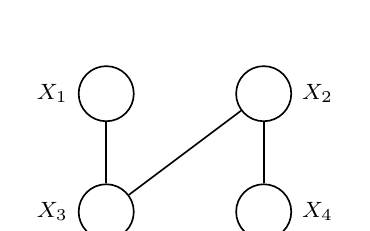
\begin{tikzpicture}[auto, node distance = 1.5cm and 2cm, on grid, semithick, state/.style ={circle, top color = white, draw, text = black, minimum width=0.7cm}, sh/.style={shade, shading = axis, left color = gray, shading angle = 45}]
\node[state, label = left:{$X_1$}] (A) {};
\node[state, label = right:{$X_2$}] (B) [right = of A] {};
\node[state, label = left:{$X_3$}] (C) [below = of A] {};
\node[state, label = right:{$X_4$}] (D) [below = of B] {};
\path (A) edge node {} (C)
(B) edge node {} (C)
(B) edge node {} (D);          
\end{tikzpicture}

\subsection{DGM}

Given the two directed graphical models, it is possible to have
a distribution $p$ on $X_1 , \cdots , X_{16}$ such that $p \in \mathcal{L}(G_1)$ and $p \in \mathcal{L}(G_2)$. Namely, take 
\begin{align}
p(x_1 , \cdots , x_{16}) = \prod_{i=1}^{16}p(x_i)
\end{align}

This is trivially in $\mathcal{L}(G_1)$ and $\mathcal{L}(G_2)$, as needed.

\section{EM algorithm}

Let $X \in \{0, 1\}^L$. Let $Z \in \{0, 1\}$ be a Bernouilli latent variable  with $p(z = 1) = \pi$. Our NB model is
$p(X_l = 1|Z = 1) = \theta_1$ and $p(X_l = 1|Z = 0) = \theta_0$, where $X = (X_1, \cdots, X_L)$ and the $X_l$'s are conditionally independent given $\theta_z$.
Suppose that we have n i.i.d. observations $\{X^{(i)}\}_{i=1}^n$ from this model. We want to estimate parameters $(\pi, \theta_0, \theta_1)$ by maximum likelihood via the EM algorithm.

The full graphical model is as follows:
\\

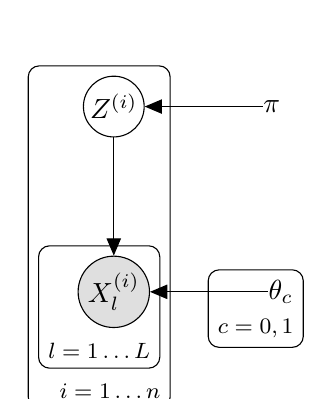
\begin{tikzpicture}[x=1.5cm,y=1.5cm]

% Define nodes
\node[obs] (x) {$X_l^{(i)}$};
\node[latent, above =of x] (z) {$Z^{(i)}$};
\node[const, right =of z] (p) {$\pi$};
\node[const, right =of x] (t) {$\theta_c$};
% Connect the nodes
\edge {z} {x};
\edge {p} {z};
\edge {t} {x};

% Plates
\plate {pl} {(x)} {$l=1\dots L$} ;
\plate {pl2} {(pl)(z)} {$i=1\dots n$} ;
\plate {pl3} {(t)} {$c=0,1$} ;
\end{tikzpicture}
\\

We derive the EM algorithm to estimate $\theta=(\pi, \theta_0, \theta_1)$. 
Let $\tau_i=p(Z^{(i)}=1\mid X^{(i)})$, $\tau=\sum_{i=1}^n \tau_i$ and $c_i = \sum_{l=1}^L X_{l}^{(i)}$. For the E-Step, given $\theta_0, \theta_1, \pi$ from the previous iteration, we would compute $\tau_i$ using the following formula:
\begin{align}
\tau_i &= p(Z^{(i)}=1\mid X^{(i)})\\
&=\frac{p(X^{(i)} \mid Z^{(i)}=1)p(Z^{(i)}=1)}{\sum_{c=0}^1 p(X^{(i)} \mid Z^{(i)}=c)p(Z^{(i)}=c)}\\
&= \frac{\prod_{l=1}^L p(X^{(i)}_l \mid Z^{(i)}=1)p(Z^{(i)}=1)}{\sum_{c=0}^1 \prod_{l=1}^L p(X^{(i)}_l \mid Z^{(i)}=c)p(Z^{(i)}=c)}\\
&=\frac{\pi\theta_1^{c_i}(1-\theta_1)^{L-c_i}}{\pi\theta_1^{c_i}(1-\theta_1)^{L-c_i} + (1-\pi)\theta_0^{c_i}(1-\theta_0)^{L-c_i}}\\
&=\frac{1}{1 +  \frac{(1-\pi)\theta_0^{c_i}(1-\theta_0)^{L-c_i}}{ \pi\theta_1^{c_i}(1-\theta_1)^{L-c_i}}}\\
&= \sigma\left(\log \frac{\pi\theta_1^{c_i}(1-\theta_1)^{L-c_i}}{(1-\pi)\theta_0^{c_i}(1-\theta_0)^{L-c_i}}\right)
\end{align}

For the M-Step, we compute $\theta_0, \theta_1, \pi$ via maximum likelihood using the $\tau_i$'s from the previous step. To simplify notation the computations we introduce an index $c$ to indicate class i.e. $\tau_{ic}=p(Z^{(i)}=c\mid X^{(i)})$ and $\pi_{c}=p(Z^{(i)}=c)$ and proceed with the understanding that $\tau_{i1}=\tau_i$ and $\pi_{i1} = \pi_i$. The objective function to optimize is as follows:
\begin{align}
\mathbb{E}\left( \ln p(X,Z,\theta) \right)=\sum_{i=1}^n \sum_{c=0}^1 \tau_{ic} [\ln \pi_c + c_i \ln \theta_c + (L-c_i)\ln(1-\theta_c)]
\end{align}

To find the maximum w.r.t. \(\pi = \pi_1\) we take derivative of (3.7) with the following term added to maintain the constraint: $\lambda (\sum_{c=0}^1 \pi_c - 1)$. This gives us:
\begin{align}
\frac{\partial}{\partial \pi_1}\mathbb{E}\left( \ln p(X,Z,\theta) \right)&=\sum_{i=1}^n \frac{\tau_{i1}}{\pi_1} - \lambda = 0\\
&\Rightarrow \pi_1 = \frac{\sum_{i=1}^n \tau_{i1}}{\lambda}
\end{align}
And satisfying the constraint gives us: $\lambda = \sum_{c=0}^1 \sum_{i=1}^n \tau_{ic} = \sum_{i=1}^n 1 = n$

Finally 
\begin{align}
\pi = \frac{\sum_{i=1}^n \tau_{i}}{n} = \frac{\tau}{n}
\end{align}

To find the maximum w.r.t. \(\theta_c\) we take derivative of (3.7). This gives us:
\begin{align}
\frac{\partial}{\partial \theta_c}\mathbb{E}\left( \ln p(X,Z,\theta) \right)&=\sum_{i=1}^n \tau_{ic} \left[\frac{c_i}{\theta_c}-\frac{L-c_i}{1-\theta_c}\right]=0\\
&\Rightarrow \sum_{i=1}^n c_i\tau_{ic} = \sum_{i=1}^n L\theta_c\tau_{ic}\\
&\Rightarrow \theta_c = \frac{\sum_{i=1}^n c_i\tau_{ic}}{L\sum_{i=1}^n \tau_{ic}}
\end{align}

Finally, after some algebra:
\begin{align}
\theta_0 &= \frac{\sum_{i=1}^n (1-\tau_i)c_i}{(n-\tau)L}\\
\theta_1 &= \frac{\sum_{i=1}^n \tau_{i}c_i}{\tau L}
\end{align}

\section{Parallel Chains}

We are given a graph and variables $X_s$ and $Y_s$ which are discrete K-valued for $s = 1, \cdots, S$, and $Z$ is a binary random variable. We are given the following factors for a specific distribution $p\in \mathcal{L}(G)$:
\begin{enumerate}
	\item $p(X_1 = l) = p(Y_1 = l) = \pi_l$ for $l = 1, \cdots , K$
	\item $p(X_s = i | X_{s-1} = j) = p(Y_s = i | Y_{s-1} = j) = A_{ij}$ for $i, j = 1, \cdots , K$ and $s = 2, \cdots, S$
	\item $p(Z = 1|X_s = k, Y_s = l) = \begin{cases}
	p & \text{if $k=l$}\\
	q & \text{o.w.}
	\end{cases}$
\end{enumerate}

We have that 
\begin{align}
p(Z=1) = \sum_{i,j} P \circ (A^{S-1}\pi)(A^{S-1}\pi)^T
\end{align}

Where 

$P\in\mathbb{R}^{K\times K}$ and $P_{ij} = \begin{cases}p & i=j \\
q & i\ne j\end{cases}$
\\

We first prove that $p(X_s=i)=[A^{S-1}\pi]_i$.  For $s=2$,
\begin{align*}
p(X_2=i) &= \sum_{j=1}^{K}p(X_2=i|X_1=j)p(X_1=j) \\
&=\sum_{j=1}^{K}A_{ij}\pi_j = [A\pi]_i
\end{align*}
Then, by induction,
\begin{align*}
p(X_S=i) &= \sum_{j=1}^{K}p(X_S=i|X_{S-1}=j)p(X_{S-1}=j) \\
&= \sum_{j=1}^{K}A_{ij}A_{ij}^{S-2}\pi\\
&= \sum_{j=1}^{K}A_{ij}^{S-1}\pi = [A^{S-1}\pi]_i
\end{align*}
Putting it all together:
\begin{align*}
p(Z=1) &= \sum_{i=1}^{k}\sum_{i=1}^{j}p(Z=1,X_s=i,Y_s=j)\\
&=\sum_{i=1}^{k}\sum_{i=1}^{j}p(Z=1|X_s=i,Y_s=j)p(X_s=i)p(Y_s=j)\\
&=\sum_{i=1}^{k}\sum_{i=1}^{j} P \circ (A^{S-1}\pi)(A^{S-1}\pi)^T
\end{align*}

\section{Metropolized Gibbs sampler}

Let $p$ be a strictly positive distribution of the random variable
$X = (X_1 , \cdots , X_n)$, with $X_i$ are K-valued random variables, with $K \ge 3$ and $p_i( z_i | x^t_{-i} ) := P(X_i = z_i | X_{-i} = x^t_{-i} )$.

We have that the Metropolized Gibbs sampler makes a proposal drawn from
the transition $q_i$ with

\begin{align}
q_i( (z_i, x^t_{-i})| (x^t_i, x^t_{-i})) := \begin{cases}
\frac{p_i( z_i | x^t_{-i} )}{1-p_i( x^{t}_i | x^t_{-i} )} & \text{for } z_i \ne x^t_{i}\\ 0 & \text{for } z_i = x^t_{i}
\end{cases}
\end{align}

\begin{enumerate}
	\item We find the acceptance probability $\alpha_i ((z_i , x^t_{i} )|(x^t_{i} ,x^t_{-i}))$ that arises from this proposal distribution $q_i$ in a Metropolis-Hasting algorithm for the target distribution $p$. For $z_i \ne x_i^{t}$ we have that:
	\begin{align*}
	\frac{q_i((x^t_i, x^t_{-i})| (z_i, x^t_{-i}))p(z_i,x^t_{-i}) }{q_i( (z_i, x^t_{-i})| (x^t_i, x^t_{-i}))p(x^t_{i} ,x^t_{-i})}
	&= \frac{p_i( x^{t}_i | x^t_{-i} )p(z_i,x^t_{-i})}{1-p_i( z_t | x^t_{-i} )}\frac{1-p_i( x^{t}_i | x^t_{-i} )}{p_i( z_i | x^t_{-i} )p(x^{t}_i,x^t_{-i})}\\
	&=\frac{1-p_i( x^{t}_i | x^t_{-i} )}{1-p_i( z_t | x^t_{-i} )}\frac{p_i( x^{t}_i | x^t_{-i} )p(z_i|x^t_{-i})p(x^t_{-i})}{p_i( z_i | x^t_{-i} )p(x^{t}_i|x^t_{-i})p(x^t_{-i})}\\
	&=\frac{1-p_i( x^{t}_i | x^t_{-i} )}{1-p_i( z_t | x^t_{-i} )}
	\end{align*}
	
	And so
	\begin{align*}
	\alpha_i ((z_i , x^t_{i} )|(x^t_{i} ,x^t_{-i})) = \min\left(1, \frac{1-p_i( x^{t}_i | x^t_{-i} )}{1-p_i( z_t | x^t_{-i} )}\right)
	\end{align*}
	
	\item We consider using a cyclic scan Gibbs sampler that samples each variable $X_i$ in a cyclic order. The Markov Chain produced by the Metropolized Gibbs sampler has $p$ as a stationary distribution because the detailed balance equation is satisfied by the construction of $\alpha_i$. $p$ is unique because the transition kernel $A_{ij}$ is regular. It is obvious that $A_{ij}>0 \forall i \ne j$, but $A_{ii}>0$ too since $A_{ii} = \sum_{z_i \ne x^t_{i}} q_i( (z_i, x^t_{-i})| (x^t_i, x^t_{-i}))(1-\alpha_i ((z_i , x^t_{i} )|(x^t_{i} ,x^t_{-i})))>0$.
\end{enumerate}

\section{Bayesian point estimates: posterior mean vs. MAP for exponential family}

We have an i.i.d sample $(x_1, \cdots, x_n)$ of Bernoulli random variables whose unknown mean parameter is \(\mathbb{E}_{X\sim p(\cdot | \mu)}\{X\} = \mu\)

\begin{enumerate}
	\item We want to compute the posterior mean estimate as a function of $\bar{x}$
	We first compute $p(\mu | x_1, \cdots, x_n)$. Notice that:
	\begin{align}\label{eq:beta}
	p(\mu | x_1, \cdots, x_n) \propto p(x_1, \cdots, x_n | \mu)p(\mu) &= \mu^{n\bar{x}}(1-\mu)^{n-n\bar{x} }\cdot 1
	\end{align}
	We recognize (\ref{eq:beta}) as a Beta distribution with $\alpha = n\bar{x} + 1$ and $\beta = n - n\bar{x} + 1$ i.e.
	\begin{align}
	p(\mu | x_1, \cdots, x_n) = \frac{\Gamma(n+2)}{\Gamma(n \bar{x}+1)\Gamma(n - n \bar{x}+1)}\mu^{n\bar{x}}(1-\mu)^{n-n\bar{x}}
	\end{align}
	Therefore,
	
	\begin{align}
	\mathbb{E}_{\mu\sim p(\cdot | X)}\{\mu\} = \frac{n \bar{x}+1}{n \bar{x}+1 + n - n \bar{x}+1}=\frac{n \bar{x}+1}{n + 2}
	\end{align}
	
	\item Since the prior is uniform, we have that the MAP estimate for \(\mu\) is the MLE. We find the MLE using stationary points by differentiating the $\log$ (for computational convenience). We get
	\begin{align*}
	\frac{\partial \log p(\mu | x_1, \cdots, x_n)}{\partial \mu} &= \frac{n\bar{x}}{\mu} - \frac{n - n\bar{x}}{1-\mu} = 0\\
	&\Rightarrow n\bar{x} - \mu n\bar{x} - \mu n + \mu n\bar{x} = 0 \\
	&\Rightarrow n\bar{x} = \mu n \\
	&\Rightarrow \mu = \bar{x}
	\end{align*}
	
	\item We express the canonical parameter $\eta$ of a Bernouilli as a function of its moment parameter $\mu$.
	\begin{align}
	p(x| \mu) = \exp\left\{ x\log \frac{\mu}{1-\mu} + \log(1-\mu) \right\}
	\end{align}
	
	Which we can write as
	\begin{align}
	p(x| \eta) = \exp\left\{ T(x)\eta - A(\eta) \right\}h(x)
	\end{align}
	Where
	\begin{align*}
	&T(x)=x \\
	&\eta = \log \frac{\mu}{1-\mu} \\
	&A(\eta)=-\log(1-\mu)=\log(1+e^{\eta}) \\
	&h(x)=1
	\end{align*}
	Note from the above $\eta = \log \frac{\mu}{1-\mu} \Rightarrow \mu = \sigma(\eta)$. 
	
	To compute $p_{\eta}(\eta)$ we use the following increasing transformation $\eta = g(\mu)$ (notice $g^{-1}(\eta) = \sigma(\eta)$). We see that:
	\begin{align*}
	p_{\eta}(\eta) &= p_{\mu}(g^{-1}(\eta))\left|\frac{dg^{-1}(\eta)}{d\eta}\right| \\
	&= p_{\mu}(\sigma(\eta))\left|\frac{d\sigma(\eta)}{d\eta}\right| \\
	&= 1 \cdot \sigma(\eta)(1-\sigma(\eta))
	\end{align*}
	As needed.
	\item The posterior mean estimate is
	\begin{align*}
	\int \mu(\eta)p(\eta| x_1, \cdots, x_n)d\eta &= \int \sigma(\eta)\frac{p( x_1, \cdots, x_n | \eta)p(\eta)}{p(x_1, \cdots, x_n)}d\eta \\
	&= \int \sigma(\eta)\frac{p( x_1, \cdots, x_n | \eta)}{p( x_1, \cdots, x_n)} \underbrace{\sigma(\eta)(1-\sigma(\eta)) d\eta}_{=d\mu}\\
	&=\int \mu \underbrace{\frac{p( x_1, \cdots, x_n | \mu)}{p( x_1, \cdots, x_n)}p(\mu)}_{=p(\mu | x_1, \cdots, x_n)}d\mu \\
	&=\mathbb{E}_{\mu\sim p(\cdot | X)}\{\mu\} \\
	&=\frac{n \bar{x}+1}{n + 2}
	\end{align*}
	
	\item Again, the MAP estimator is the MLE, since the prior is uniform. We use that the MLE is a plug in estimator to get that $\eta^{MAP} = \log \frac{\bar{x}}{1-\bar{x}}$. Then $\mu(\eta^{MAP})= \bar{x}$.
	
	\item Note that 1. and 3. are the same because the integral is essentially the same (with the only difference being the measure). 2. and 5. are the same since the MLE is the same as MAP for a uniform prior, and the MLE is invariant to continous mappings.
	
	
\end{enumerate}

\end{document}